\documentclass[tikz,border=6pt]{standalone}

\usepackage{amsmath,amssymb}
\usetikzlibrary{calc,arrows.meta,shapes.geometric}

\begin{document}

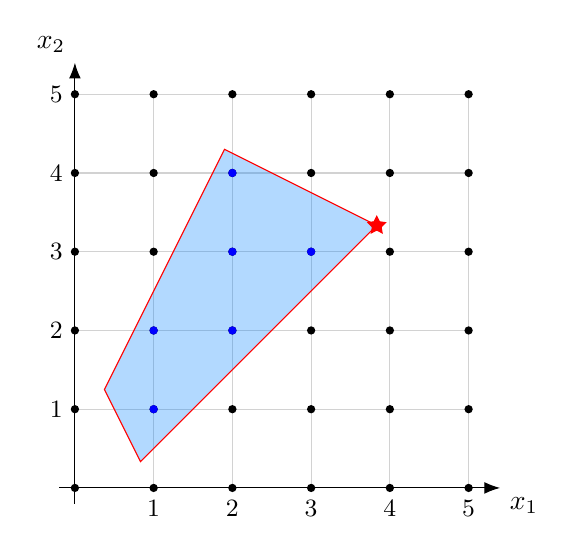
\begin{tikzpicture}[scale=1.0]
  % axes
  \draw[-{Latex[length=2mm]}] (-0.2,0) -- (5.4,0) node[below right] {$x_1$};
  \draw[-{Latex[length=2mm]}] (0,-0.2) -- (0,5.4) node[above left] {$x_2$};

  % light grid guides + tick labels (drawn first)
  \foreach \i in {1,...,5} {
    \draw[gray!35] (\i,0) -- (\i,5);
    \draw[gray!35] (0,\i) -- (5,\i);
    \node[below] at (\i,-0.03) {\small \i};
    \node[left]  at (-0.03,\i) {\small \i};
  }

  % feasible polygon (fill first so points can be drawn on top)
  % Vertices from constraint intersections:
  %  A∩D: (0.375, 1.25)
  %  C∩D: (0.833333..., 0.333333...)
  %  B∩C: (3.833333..., 3.333333...)
  %  A∩B: (1.9, 4.3)
  \def\vAD{(0.375,1.25)}
  \def\vCD{(0.833333,0.333333)}
  \def\vBC{(3.833333,3.333333)}
  \def\vAB{(1.9,4.3)}

  \fill[blue!50!cyan,opacity=0.3]
    \vAD -- \vCD -- \vBC -- \vAB -- cycle;
      \draw[red]
    \vAD -- \vCD -- \vBC -- \vAB -- cycle;

  % --- Lattice points: draw AFTER the polygon so they are in front
  \foreach \i in {0,...,5} {
    \foreach \j in {0,...,5} {
      \fill[black] (\i,\j) circle (1.5pt);
    }
  }

  % Feasible integer grid points (green), drawn last so they sit on top
  \foreach \P in {(1,1),(1,2),(2,2),(2,3),(3,3),(2,4)}{
    \fill[blue] \P circle (1.5pt);
  }

  % LP optimum (blue star) at B∩C, shrunk to half size
  \node[star,star points=5,star point ratio=2.0,fill=red,draw=red,scale=0.35]
    at \vBC {};

%  % model printed below the plot
%  \node[anchor=north west] at (-0.05,-0.85) {%
%    $\begin{aligned}
%      \max\quad & x_1 + x_2\\
%      \text{s.t.}\quad
%      & -2x_1 + x_2 \le 0.5,\\
%      & x_1 + 2x_2 \le 10.5,\\
%      & x_1 - x_2 \le 0.5,\\
%      & -2x_1 - x_2 \le -2,\\
%      & x_1, x_2 \in \mathbb{Z}.
%    \end{aligned}$};
\end{tikzpicture}

\end{document}
